
\documentclass[a4paper,11pt]{extarticle}
\usepackage{geometry}
\usepackage{listings}
\usepackage{graphicx}
\usepackage{float} 

% Set margins
\geometry{
  a4paper,
  total={170mm,257mm},
  left=25mm,
  right=25mm,
  top=20mm,
  bottom=25mm,
}

\title{DATA422-W8-82171165 \\Assignment Submission Report}
\author{David Ewing (82171165)}
\date{2024-09-16}

\begin{document}

\maketitle

\section*{Overview}
This report outlines the deliverables required for the SQL assignment. The assignment involves interacting with a PostgreSQL database, retrieving data, visualising it, performing joins, and analysing query performance. The implementation uses an \texttt{.Renviron} file for secure database credentials and an R script to perform the various operations.

\section*{Deliverables}
We will produce code in an R script that will achieve the following objectives:
\begin{itemize}
    \item List the tables
    \item List all the fields in a table
    \item Pull some data using a query
    \item Plot the data
    \item Perform a join and pull the result
    \item Investigate an execution plan

\end{itemize}


\noindent However, the sections of the document that follow confuse what is truely meant as Deliverables. My interpretation will be as follows:
\begin{enumerate}
  \setcounter{enumi}{-1}  % This will set the first item to be numbered as 0
  \item Database Connection
  \item Listing Tables, Fields, Rows and Count
  \item Join Operation
  \item SQL Query and Line Graph of Daily Income
  \item SQL Query and Bar Graph for Inventory Stock Take
  \item Investigate an Execution Plan
\end{enumerate}

\newpage
\section*{Deliverable 0: Database Connection}
The database connection was not iterated as a deliverable in the Assignment. The database connection is established using the following environment variables stored in the \texttt{.Renviron} file:
\begin{verbatim}
PG_HOST = mathmads.canterbury.ac.nz
PG_PORT = 8909
PG_USR = student_data422
PG_PASS = readonly
\end{verbatim}
The R script connects to the PostgreSQL database securely by referencing these environment variables.
\begin{verbatim}
> #
> #-------------------------------------------------------------------------------
> # DELIVERABLE 0: Database Connection
> #  environment variables (CONFIRM in environment values)
> #
> dbname <- Sys.getenv("PG_DBNAME", "Jeff")
> host <- Sys.getenv("PG_HOST", "mathmads.canterbury.ac.nz")
> port <- Sys.getenv("PG_PORT", "8909")
> user <- Sys.getenv("PG_USR", "student_data422")
> password <- Sys.getenv("PG_PASS") ## NO DEFAULT for security purposes. 
> #
> # connection object via environment variables (.Fenviron)
> #
> con <- dbConnect(
+   Postgres(),
+   dbname = dbname,
+   host = host,
+   port = port,
+   user = user,
+   password = password
+ )
> #
> # confirm connection status
> #
> if (!dbIsValid(con)) {
+   stop("FAILED connection to PostgreSQL database.")
+ } else {
+   print("SUCCESSFUL connection to PostgreSQL database.")
+ }
[1] "SUCCESSFUL connection to PostgreSQL database."
> 
\end{verbatim}
\newpage
\section*{Deliverable 1: Listing Tables, Fields, Rows and Count}
The assignment lists explicitly four deliverables required. The specific results:
\begin{verbatim}
> #
> #-------------------------------------------------------------------------------
> # DELIVERABLE 1.1: List all tables in the connected database
> tables <- dbListTables(con)
> print(tables)
 [1] "actor"                      "address"                    "category"                  
 [4] "city"                       "country"                    "customer"                  
 [7] "film"                       "film_actor"                 "film_category"             
[10] "inventory"                  "language"                   "payment"                   
[13] "rental"                     "staff"                      "store"                     
[16] "actor_info"                 "customer_list"              "film_list"                 
[19] "nicer_but_slower_film_list" "sales_by_film_category"     "sales_by_store"            
[22] "staff_list"                
> #
> #-------------------------------------------------------------------------------
> # DELIVERABLE 1.2: List all the fields in a table
> fields <- dbListFields(con, "rental")
> print(fields)
[1] "rental_id"    "rental_date"  "inventory_id" "customer_id"  "return_date"  "staff_id"     "last_update" 
> #
> #-------------------------------------------------------------------------------
> # DELIVERABLE 1.3: Pull some data from the 'rental' table as an example
> query <- "SELECT rental_id, rental_date, inventory_id, customer_id FROM rental LIMIT 10"
> data <- dbGetQuery(con, query)
> print(data)
   rental_id         rental_date inventory_id customer_id
1          2 2005-05-24 22:54:33         1525         459
2          3 2005-05-24 23:03:39         1711         408
3          4 2005-05-24 23:04:41         2452         333
4          5 2005-05-24 23:05:21         2079         222
5          6 2005-05-24 23:08:07         2792         549
6          7 2005-05-24 23:11:53         3995         269
7          8 2005-05-24 23:31:46         2346         239
8          9 2005-05-25 00:00:40         2580         126
9         10 2005-05-25 00:02:21         1824         399
10        11 2005-05-25 00:09:02         4443         142
> #
> #-------------------------------------------------------------------------------
> # DELIVERABLE 1.4: Pull the total number of rentals
> #
> query <- "SELECT COUNT(*) FROM rental"
> dbGetQuery(con, query)
  count
1 16044
\end{verbatim}
\newpage
\section*{Deliverable 2: Join Operation}
A SQL \texttt{JOIN} (default) is performed between the \texttt{rental} and \texttt{customer} tables, retrieving the first and last names of customers who rented items. The following SQL query is used:
\begin{verbatim}
SELECT rental.rental_id, rental.rental_date, customer.first_name, customer.last_name
FROM rental
JOIN customer ON rental.customer_id = customer.customer_id
LIMIT 10;
\end{verbatim}
Specific results:
\begin{verbatim}
> #-------------------------------------------------------------------------------
> # DELIVERABLE 2: Perform a JOIN between 'rental' and 'customer' tables to get customer names
> # INNER JOIN (SQL default):
> # JOIN customer ON rental.customer_id = customer.customer_id 
> join_query <- "
+   SELECT rental.rental_id, rental.rental_date, customer.first_name, customer.last_name
+   FROM rental
+   JOIN customer ON rental.customer_id = customer.customer_id
+   LIMIT 10
+ "
> joined_data <- dbGetQuery(con, join_query)
> print(joined_data)
   rental_id         rental_date first_name   last_name
1          2 2005-05-24 22:54:33      Tommy     Collazo
2          3 2005-05-24 23:03:39     Manuel     Murrell
3          4 2005-05-24 23:04:41     Andrew       Purdy
4          5 2005-05-24 23:05:21    Delores      Hansen
5          6 2005-05-24 23:08:07     Nelson Christenson
6          7 2005-05-24 23:11:53  Cassandra     Walters
7          8 2005-05-24 23:31:46     Minnie      Romero
8          9 2005-05-25 00:00:40      Ellen     Simpson
9         10 2005-05-25 00:02:21      Danny        Isom
10        11 2005-05-25 00:09:02      April       Burns
\end{verbatim}
\newpage
\section*{Deliverable 3: SQL Query and Line Graph of Daily Income}
The script pulls data from the \texttt{rental} table using the following SQL query:
\begin{verbatim}
SELECT 
    DATE(rental.rental_date) AS rental_date, 
    SUM(payment.amount) AS total_revenue
FROM rental
JOIN payment ON rental.rental_id = payment.rental_id
GROUP BY DATE(rental.rental_date)
ORDER BY rental_date;

> #
> #-------------------------------------------------------------------------------
> # DELIVERABLE 3: SQL Query and Line Graph of Daily Income
> #
> # SQL query to get total daily revenue
> query <- "
+ SELECT 
+     DATE(rental.rental_date) AS rental_date, 
+     SUM(payment.amount) AS total_revenue
+ FROM rental
+ JOIN payment ON rental.rental_id = payment.rental_id
+ GROUP BY DATE(rental.rental_date)
+ ORDER BY rental_date;
+ "
> # Execute the query
> revenue_data <- dbGetQuery(con, query)
> # Print the retrieved data
> print(revenue_data)
   rental_date total_revenue
1   2005-06-14         41.89
2   2005-06-15       1179.97
3   2005-06-16       1191.11
...
30  2005-08-21       2809.41
31  2005-08-22       2576.74
32  2005-08-23       2521.02
33  2006-02-14        514.18
\end{verbatim}

\begin{figure}
    \centering
    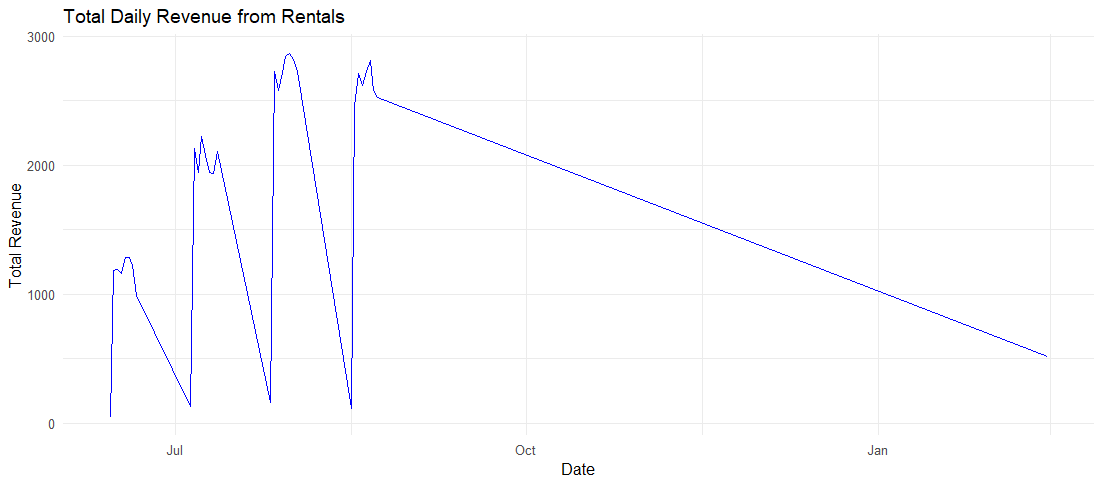
\includegraphics[width=0.7\linewidth]{line-graph.png}
    \caption{Line Graph of Daily Income}
    \label{fig:linegraph}
\end{figure}
\newpage
\begin{figure}
    \centering
    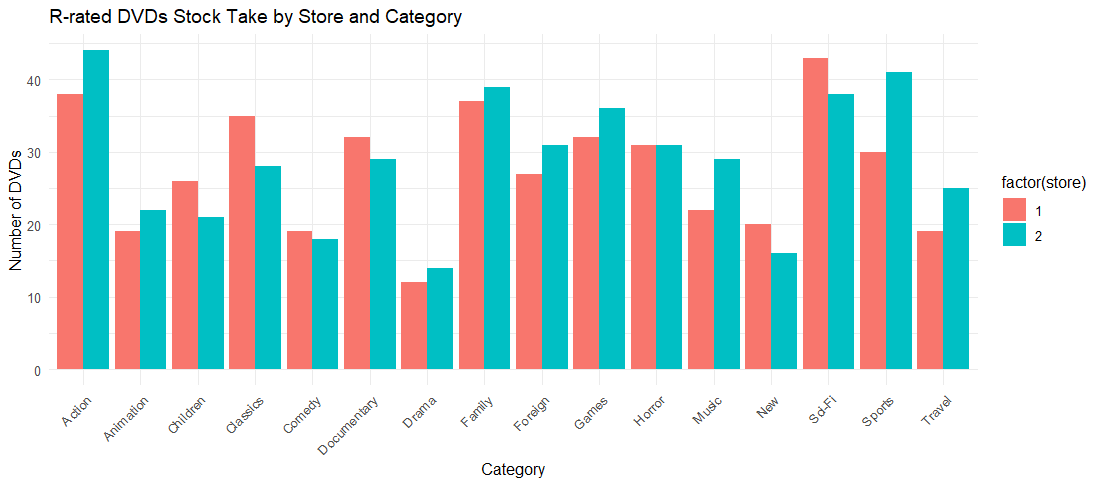
\includegraphics[width=0.7\linewidth]{bar-graph.png}
    \caption{Bar Graph for Inventory Stock Take}
    \label{fig:enter-label}
\end{figure}
\section*{Deliverable 4: SQL Query and Bar Graph for Inventory Stock Take}
The script pulls data from the \texttt{rental} table using the following SQL query:
\begin{verbatim}
WITH r_rated_movies AS (
    SELECT 
        film.film_id, 
        film.title, 
        film.rating, 
        film_category.category_id, 
        inventory.store_id
    FROM film
    JOIN film_category ON film.film_id = film_category.film_id
    JOIN inventory ON film.film_id = inventory.film_id
    WHERE film.rating = 'R'
)
SELECT 
    store.store_id AS store, 
    category.name AS category, 
    COUNT(r_rated_movies.film_id) AS dvd_count
FROM r_rated_movies
JOIN store ON r_rated_movies.store_id = store.store_id
JOIN category ON r_rated_movies.category_id = category.category_id
GROUP BY store.store_id, category.name
ORDER BY store.store_id, category.name;
\end{verbatim}

\newpage
\begin{verbatim}
> #-------------------------------------------------------------------------------
> # DELIVERABLE 4: SQL query and Bar Graph for Inventory Stock Take
> # Requirements for the Inventory Stock Take:
> #  1. Aliasing of variable names: Use SQL aliases to simplify table and column references.
> #  2. Common Table Expression (CTE): Use a CTE for organising part of the query.
> #  3. Five Joins: Join at least five tables in the query.
> #  4. Where statement: Filter the data (in this case, to focus on R-rated movies).
> #  5. Group by: Group the data (by store and movie category).
> #  6. Aggregating function: Use an aggregation function (such as COUNT()) to count DVDs.
> #
> query <- "
+ WITH r_rated_movies AS (
+     SELECT 
+         film.film_id, 
+         film.title, 
+         film.rating, 
+         film_category.category_id, 
+         inventory.store_id
+     FROM film
+     JOIN film_category ON film.film_id = film_category.film_id
+     JOIN inventory ON film.film_id = inventory.film_id
+     WHERE film.rating = 'R'
+ )
+ SELECT 
+     store.store_id AS store, 
+     category.name AS category, 
+     COUNT(r_rated_movies.film_id) AS dvd_count
+ FROM r_rated_movies
+ JOIN store ON r_rated_movies.store_id = store.store_id
+ JOIN category ON r_rated_movies.category_id = category.category_id
+ GROUP BY store.store_id, category.name
+ ORDER BY store.store_id, category.name;
+ "
> # Execute the query
> stock_data <- dbGetQuery(con, query)
> # Print the data
> print(stock_data)
   store    category dvd_count
1      1      Action        38
2      1   Animation        19
3      1    Children        26
4      1    Classics        35
...
25     2     Foreign        31
26     2       Games        36
27     2      Horror        31
28     2       Music        29
29     2         New        16
30     2      Sci-Fi        38
31     2      Sports        41
32     2      Travel        25

\end{verbatim}



\newpage
\section*{Deliverable 5: Investigate an Execution Plan}
An \texttt{EXPLAIN} statement is executed to analyse the performance of the \texttt{JOIN} query. The query plan is printed as follows:
\begin{verbatim}
EXPLAIN SELECT rental.rental_id, rental.rental_date, customer.first_name, 
   customer.last_name
FROM rental
JOIN customer ON rental.customer_id = customer.customer_id;
\end{verbatim}
Specific Results:
\begin{verbatim}
> #-------------------------------------------------------------------------------
> # Investigate the execution plan for the JOIN query
> # results are in dataframe 
> explain_query <- "
+   EXPLAIN SELECT rental.rental_id, rental.rental_date, customer.first_name, 
customer.last_name 
+   FROM rental
+   JOIN customer ON rental.customer_id = customer.customer_id
+ "
> execution_plan <- dbGetQuery(con, explain_query)
> print(execution_plan)
                                                              QUERY PLAN
1                    Hash Join  (cost=22.48..375.33 rows=16044 width=25)
2                 Hash Cond: (rental.customer_id = customer.customer_id)
3        ->  Seq Scan on rental  (cost=0.00..310.44 rows=16044 width=14)
4                        ->  Hash  (cost=14.99..14.99 rows=599 width=17)
5         ->  Seq Scan on customer  (cost=0.00..14.99 rows=599 width=17)
\end{verbatim}
\section*{Conclusion}
The \texttt{.Renviron} file and \texttt{00\_submission.R} script together fulfil all the deliverables for this assignment, including secure database access, querying data, visualising results, and analysing query performance.

\end{document}
